% Copyright 2026 Sreeram Anil
% SPDX-License-Identifier: CC-BY-4.0
% =============================================================================
%  Direct neural SOC regression (NN-Direct)
% =============================================================================
\chapter{Direct neural state-of-charge regression (NN-Direct)}
\label{ch:nndirect}

\section*{At a glance}
\begin{tabular}{@{}l>{\raggedright\arraybackslash}p{0.76\textwidth}@{}}
Family & learning (data-driven) \\
Header & \texttt{include/estkit/learning/nn\_direct.hpp}, \texttt{mlp.hpp}, \texttt{train\_data.hpp} \\
Registered name & \texttt{NN-Direct} \\
State dimension & none --- the method has no state-space model; $n_\phi = 8$ input features \\
Cost per step & $\num{288}$ multiply--accumulates $+$ $32$ \texttt{tanh};
$\approx\SI{0.4}{\micro\second}$, no heap \\
Memory & \SI{12.3}{\kilo\byte} boxcar buffers $+$ \SI{2.6}{\kilo\byte} weights \\
Primary references & \cite{chemali2018dnn,hornik1989,kingma2015adam,rumelhart1986backprop} \\
\end{tabular}

\section{Motivation and aerospace/BMS relevance}
Every estimator in the preceding chapters is \emph{model-based}: it owns an equivalent-circuit
model of the cell, and its accuracy is bounded by how well that model describes the specimen in
front of it.  Building that model is expensive.  It requires a characterisation campaign
(pulse tests at several temperatures and states of charge, an OCV sweep at $C/25$, a capacity
check), it has to be repeated for every chemistry and every form factor, and it has to be
maintained as the cell ages.  The obvious question --- and the one the machine-learning
literature on battery management has been asking since about 2016 --- is whether the
characterisation campaign can be replaced by a regression fitted directly to logged flight or
drive-cycle data.

\citet{chemali2018dnn} answer it affirmatively for automotive duty cycles: a deep feedforward
network that takes the measured terminal voltage, current and temperature, together with their
running averages, and emits the state of charge, reaches roughly \SI{1}{\percent} mean absolute
error across a range of ambient temperatures with no cell model, no OCV table, no Coulomb
counter and no filter.  The appeal for a battery management system is real: the inference path is
a fixed sequence of multiply--accumulates, it is branch-free, it has an exactly predictable
execution time, and it needs neither a matrix inverse nor a square root.

The appeal for an \emph{airborne} battery management system is much weaker, and understanding
precisely why is the purpose of this chapter.  A learned regressor is only defined on the data
distribution it was trained on.  The eVTOL mission of this benchmark reaches
4.5\,C during hover, with manoeuvre pulses to about \SI{29}{\ampere}; the fixed-wing and
hover-hold missions used for training reach only 3.0\,C and 3.5\,C.  The
network is therefore asked to \emph{extrapolate} in the one variable --- current --- that
dominates the ohmic term of the terminal voltage.  It is exactly this situation that the
certification guidance for machine-learning items is written around: \citet{easa2023ai} requires
an explicit \emph{operational design domain} and evidence that the item is never operated outside
it, while \citet{rtca2011do178c} assumes a specification against which the code can be verified
--- a specification that a table of $\num{321}$ fitted weights does not provide.  This chapter is
therefore included as the honest counter-example in a library of model-based estimators: it is
implemented carefully, trained properly, and measured against the same eleven fault scenarios as
everything else.

\section{Problem statement and assumptions}
Let $z_k \in [0,1]$ denote the true state of charge at sample $k$, and let the measured signals be
the terminal voltage $v_k$ [\si{\volt}], the current $i_k$ [\si{\ampere}, discharge positive] and
the cell temperature $T_k$ [\si{\kelvin}].  The method assumes:

\begin{assumption}[Static map]\label{as:nnd-static}
There exists a function $\mathcal{N}$ and a finite feature window such that
$z_k = \mathcal{N}(\phi_k) + e_k$ with $\E{e_k}\approx 0$, where $\phi_k$ is built from
$\{v_j, i_j, T_j\}_{j\le k}$ only.
\end{assumption}

\begin{assumption}[Coverage]\label{as:nnd-cover}
The joint distribution of $\phi_k$ during operation is contained in the support of the training
distribution.
\end{assumption}

Assumption~\ref{as:nnd-static} is not innocuous.  The state of charge is an \emph{integrator} of
the current; no finite-window static map of the measurements can reproduce it exactly, because two
missions with identical recent history but different histories before the window have different
SOC.  The Coulomb-count feature of \cref{eq:nnd-cc} below is what makes the assumption
approximately true: it carries the integral explicitly.  Assumption~\ref{as:nnd-cover} is the one
the benchmark deliberately violates.

By the universal-approximation theorem \citep{hornik1989}, a single hidden layer with enough
\texttt{tanh} units can approximate any continuous $\mathcal{N}$ on a compact set to arbitrary
accuracy; the theorem says nothing at all about behaviour off that set, nor about how many samples
are needed to \emph{find} the approximation.

\section{Derivation}

\subsection{Features}
The feature vector follows \citet{chemali2018dnn}: instantaneous voltage, current and temperature
plus moving averages that give the network access to the recent dynamics, and --- specific to
this implementation --- the Coulomb count, which supplies the integral information
Assumption~\ref{as:nnd-static} needs:
\begin{equation}\label{eq:nnd-feat}
\phi_k = \bigl[\, v_k,\; i_k,\; T_k,\; \langle v\rangle^{10}_k,\; \langle v\rangle^{60}_k,\;
\langle i\rangle^{10}_k,\; \langle i\rangle^{60}_k,\; \Delta z^{\mathrm{CC}}_k \,\bigr]^\T
\in\real^{8},
\end{equation}
where the boxcar (sliding-window) mean over a window of $W$ seconds is
\begin{equation}\label{eq:nnd-box}
\langle x\rangle^{W}_k = \frac{1}{N_W}\sum_{j=k-N_W+1}^{k} x_j,\qquad N_W = \operatorname{round}(W/\dt),
\end{equation}
(for $k < N_W$ the average is taken over the samples available so far), and the Coulomb-count
increment since the estimator was reset is
\begin{equation}\label{eq:nnd-cc}
\Delta z^{\mathrm{CC}}_k = -\sum_{j<k} \frac{\eta(i_j)\, i_j\, \dt}{3600\, Q_{\mathrm{nom}}},
\qquad
\eta(i) = \begin{cases} 1 & i \ge 0\\ \eta_c & i<0,\end{cases}
\end{equation}
with $Q_{\mathrm{nom}}$ the nameplate capacity in \si{\ampere\hour} \citep{ng2009coulomb}.  Note
that $\Delta z^{\mathrm{CC}}_k$ uses only samples strictly before $k$, so \cref{eq:nnd-feat} is
causal and contains no information from the future.

\subsection{Network}
With $n_\phi = 8$ inputs, $n_h = 32$ hidden units and one output, and with per-feature
standardisation folded into the object \citep{bishop1995nn},
\begin{align}
s_{k,m} &= \frac{\phi_{k,m} - \mu_m}{\sigma_m}, & m &= 1\ldots n_\phi, \label{eq:nnd-std}\\
a_{k,j} &= \tanh\Bigl(\textstyle\sum_{m} W^{(1)}_{jm} s_{k,m} + b^{(1)}_j\Bigr), & j &= 1\ldots n_h,
\label{eq:nnd-hidden}\\
g_k     &= \textstyle\sum_j W^{(2)}_{j} a_{k,j} + b^{(2)}, \label{eq:nnd-out}\\
\hat z_k &= \operatorname{clip}_{[-0.05,\,1.05]}\bigl(\mu^y + \sigma^y g_k\bigr), \label{eq:nnd-desc}
\end{align}
where $\mu_m,\sigma_m$ are the empirical mean and standard deviation of feature $m$ over the
training set and $\mu^y,\sigma^y$ those of the target.  The parameter vector is
$\theta = \{W^{(1)}, b^{(1)}, W^{(2)}, b^{(2)}\}$ with
$n_\theta = n_h n_\phi + n_h + n_h + 1 = \num{321}$ entries; with $n_h=32$ this gives
$\num{321}$ parameters, stored as \texttt{Real} together with $2(n_\phi + 1) = 18$ standardisation
constants.

Standardisation is not cosmetic.  The raw features span
$v\sim\SI{3.5}{\volt}$, $i\sim\SI{10}{\ampere}$, $T\sim\SI{25}{\celsius}$ and
$\Delta z^{\mathrm{CC}}\sim 0.3$; without \cref{eq:nnd-std} the first-layer gradients differ by
three orders of magnitude between inputs and \texttt{tanh} saturates on the voltage channel at
initialisation.

\subsection{Loss and gradients}
Training minimises the mean squared error in \emph{standardised} output units over the $N$
training samples,
\begin{equation}\label{eq:nnd-loss}
L(\theta) = \frac{1}{2N}\sum_{n=1}^{N}\bigl(g(\phi^{(n)};\theta) - t^{(n)}\bigr)^2
+ \frac{\lambda_2}{2}\norm{\theta}^2,
\qquad t^{(n)} = \frac{z^{(n)} - \mu^y}{\sigma^y},
\end{equation}
with a weak ridge term $\lambda_2 = \num{e-6}$.  Backpropagation \citep{rumelhart1986backprop}
through \crefrange{eq:nnd-std}{eq:nnd-out} gives, per sample, with $e = g - t$,
\begin{equation}\label{eq:nnd-grad}
\frac{\partial L}{\partial W^{(2)}_j} = e\, a_j,\quad
\frac{\partial L}{\partial b^{(2)}} = e,\quad
\delta_j = (1 - a_j^2)\, W^{(2)}_j e,\quad
\frac{\partial L}{\partial W^{(1)}_{jm}} = \delta_j s_m,\quad
\frac{\partial L}{\partial b^{(1)}_j} = \delta_j ,
\end{equation}
where $1-a_j^2 = \tanh'$ costs nothing extra because $a_j$ is already available.

\subsection{Optimiser}
Parameters are updated by Adam \citep{kingma2015adam} on mini-batches of $B=32$:
\begin{align}
m_t &= \beta_1 m_{t-1} + (1-\beta_1) g_t, &
v_t &= \beta_2 v_{t-1} + (1-\beta_2) g_t^{\odot 2}, \label{eq:nnd-adam1}\\
\hat m_t &= \frac{m_t}{1-\beta_1^t}, &
\hat v_t &= \frac{v_t}{1-\beta_2^t}, \label{eq:nnd-adam2}\\
\theta_t &= \theta_{t-1} - \alpha_e\, \hat m_t \oslash \bigl(\sqrt{\hat v_t} + \epsilon\bigr), &&
\label{eq:nnd-adam3}
\end{align}
with $\beta_1 = 0.9$, $\beta_2 = 0.999$, $\epsilon = \num{e-8}$ and a \emph{decaying} step size
\begin{equation}\label{eq:nnd-lr}
\alpha_e = \alpha_0\, \kappa^{\,e/(E-1)},\qquad \alpha_0 = \num{6e-3},\ \kappa = 0.05,\ E = 20 .
\end{equation}
The decay in \cref{eq:nnd-lr} is a \emph{determinism} requirement, not a convergence trick.  With a
constant Adam step the parameters keep bouncing inside the minimum and the weights one happens to
stop at depend on the epoch count: in a single-seed development experiment, training the same
network on the same data for $10$, $20$ and $25$ epochs produced steady-state benchmark errors of
\SI{1.20}{}, \SI{2.10}{} and \SI{0.86}{\percent} SOC --- a factor of $2.4$ of pure optimiser
jitter, and one setting that would have failed the \SI{2}{\percent} acceptance threshold outright.
With \cref{eq:nnd-lr} the same sweep gives \SI{1.29}{}, \SI{1.04}{} and \SI{1.03}{\percent},
monotone and reproducible.  A qualification argument that cannot state \emph{which} weights will be
delivered is not an argument at all.

\subsection{Weight initialisation and sample order}
Weights are drawn once from the deterministic \texttt{xoshiro256**} stream
\citep{blackman2021xoshiro} using the Glorot uniform rule \citep{glorot2010init},
$W^{(\ell)}_{ij}\sim \mathcal{U}(-\gamma_\ell,\gamma_\ell)$ with
$\gamma_\ell = \sqrt{6/(\mathrm{fan_{in}}+\mathrm{fan_{out}})}$, biases at zero.  Mini-batch order
is randomised without a heap-allocated permutation: each epoch visits the samples along the cyclic
sequence $\mathrm{idx}_t = (o + t s) \bmod N$ with a random offset $o$ and a random stride $s$
coprime to $N$.  Because $\gcd(s,N)=1$ this is a bijection of $\{0,\dots,N-1\}$, so every sample is
seen exactly once per epoch, the order differs between epochs, and no dynamic memory is required.

\section{Algorithm}
\begin{algorithm}[H]
\caption{NN-Direct --- offline training (once) and one on-line sample}
\begin{algorithmic}[1]
\Statex \textbf{Offline (host, once per delivered software build)}
\Require mission set $\mathcal{M}$, scenario set $\mathcal{S}$, seed set, epochs $E$, seed $\sigma_0$
\State $\mathcal{D}\gets\emptyset$
\ForAll{$(\text{mission},\text{scenario},\text{seed}) \in \mathcal{M}\times\mathcal{S}\times\text{seeds}$}
  \State simulate / log the mission; reset the feature extractor
  \For{$k = 0,\dots,n-1$} \Comment{every sample, to keep the moving averages correct}
    \State form $\phi_k$ by \crefrange{eq:nnd-feat}{eq:nnd-cc}
    \If{$k \bmod 10 = 0$} $\mathcal{D}\gets\mathcal{D}\cup\{(\phi_k, z_k)\}$ \Comment{record at \SI{1}{\hertz}} \EndIf
  \EndFor
\EndFor
\State $\mu,\sigma \gets$ mean/std of $\mathcal{D}$; initialise $\theta$ by Glorot \citep{glorot2010init}
\For{$e = 0,\dots,E-1$}
  \State $\alpha_e \gets$ \cref{eq:nnd-lr}; pick a cyclic-shuffle offset and stride
  \ForAll{mini-batches of size $B$}
    \State accumulate $\nabla_\theta L$ by \cref{eq:nnd-grad}; update $\theta$ by \crefrange{eq:nnd-adam1}{eq:nnd-adam3}
  \EndFor
\EndFor
\Statex \textbf{On-line (target, per sample)}
\Require $v_k, i_k, T_k$, frozen $\theta,\mu,\sigma$
\State push $v_k,i_k$ into the four boxcar accumulators; read $\langle\cdot\rangle^{10},\langle\cdot\rangle^{60}$
\State assemble $\phi_k$; \textbf{accumulate} $\Delta z^{\mathrm{CC}}$ \emph{after} assembling $\phi_k$
\State $s \gets (\phi_k-\mu)\oslash\sigma$; $a\gets\tanh(W^{(1)}s + b^{(1)})$; $g\gets W^{(2)}a + b^{(2)}$
\Ensure $\hat z_k = \operatorname{clip}_{[-0.05,1.05]}(\mu^y + \sigma^y g)$
\end{algorithmic}
\end{algorithm}

\section{Application to the battery model}
The training set is generated from the ECM truth plant of Chapter~\ref{ch:ecm} through
\texttt{make\_dataset}, using only the \texttt{fixed\_wing} and \texttt{hover\_hold} missions ---
\emph{never} the \texttt{evtol} mission on which the benchmark reports.  The helper
\texttt{for\_each\_training\_dataset} in \texttt{train\_data.hpp} refuses to emit an eVTOL dataset,
so the train/test split cannot be broken by a later edit.  The training conditions are the
Cartesian product of
\begin{itemize}[nosep]
  \item missions: \texttt{fixed\_wing}, \texttt{hover\_hold};
  \item scenarios: \texttt{nominal}, \texttt{cold} ($T_\text{amb}=\SI{-10}{\celsius}$),
        \texttt{hot} ($T_\text{amb}=\SI{45}{\celsius}$), \texttt{aged\_cell} (\SI{15}{\percent}
        capacity loss);
  \item truth-cell variants: with and without the Preisach hysteresis operator
        \citep{mayergoyz1991hysteresis,baronti2014hysteresis}, so that the fitted map represents a
        \emph{population} of cells rather than one specimen;
  \item three pseudo-random seeds per combination (gust realisation and sensor-noise stream).
\end{itemize}
This gives $2\times4\times2\times3 = 48$ missions; after decimation to \SI{1}{\hertz} the training
set holds $N = \num{96480}$ samples.  The inputs are the \emph{measured} signals
$i^{\text{meas}}, v^{\text{meas}}, T^{\text{meas}}$ --- including the nominal current-sensor bias
(\SI{0.02}{\ampere}), gain error (\SI{0.5}{\percent}) and ADC quantisation --- and the target is the
plant's true SOC, which is precisely the information a laboratory campaign with a reference
coulometer would produce.

The network is fitted \emph{lazily}, once per process, on the first call to \texttt{reset()};
the resulting weights are held in a function-local \texttt{static} so that every subsequent
scenario, seed and repetition reuses them.  Data generation takes \SI{0.9}{\second} and the $20$
Adam epochs a further \SI{1.4}{\second} on the two-core benchmark host --- comfortably inside the
budget, and irrelevant on the target, where the weights arrive as a constant table.

\texttt{NN-Direct} implements \texttt{estkit::Estimator} directly rather than through
\texttt{CellEstimator}: it has no state-space model, no covariance and no measurement equation, so
\texttt{soc\_std()} returns $-1$ and \texttt{voltage\_pred()} returns NaN.  The benchmark's voltage
RMSE column is therefore empty for this estimator --- itself a diagnostic observation, because a
method that cannot predict its own measurement cannot perform residual-based fault detection.

\section{Implementation notes}
\paragraph{Memory and time.}  The four boxcar accumulators dominate the footprint:
$2\times128 + 2\times640 = \num{1536}$ \texttt{Real} words, i.e.\ \SI{12.3}{\kilo\byte} in double
precision (\SI{6.1}{\kilo\byte} in the \texttt{float} build), against \SI{2.6}{\kilo\byte} for the
weights.  Each boxcar update is $\mathcal{O}(1)$ (subtract the leaving sample, add the arriving
one), so the per-sample cost is dominated by the $n_\phi n_h + n_h = \num{288}$ multiply--accumulates
of \crefrange{eq:nnd-hidden}{eq:nnd-out} plus $32$ \texttt{tanh} evaluations.  On a Cortex-M7 at
\SI{400}{\mega\hertz} with a single-precision FPU and a polynomial \texttt{tanh}, this is
$\approx\SI{3}{\micro\second}$ --- entirely affordable at \SI{10}{\hertz}.  An implementation short
of RAM would replace the boxcars by first-order exponential averages
($\langle x\rangle \leftarrow \langle x\rangle + (\dt/W)(x - \langle x\rangle)$), reducing the state
to four scalars at the cost of a slightly different (and retrainable) feature definition.

\paragraph{Determinism.}  Every source of randomness is a seed constant compiled into the header:
the weight initialisation (\texttt{init\_seed}), the mission gust and sensor streams
(\texttt{seed0}) and the mini-batch order.  Two builds of the same source therefore produce
bit-identical weights on the same compiler and rounding mode.  Inference contains no branches on
data, no iteration counts that depend on values, and no dynamic memory, so worst-case execution
time equals typical execution time --- the one genuine advantage this method has for certification.

\paragraph{\texttt{float} build.}  All arithmetic is in \texttt{Real}.  Training in single precision
is numerically acceptable here because the loss is well scaled by \cref{eq:nnd-std}; the
single-precision build reproduces the double-precision benchmark to two decimals on every scenario
of Table~\ref{tab:float} (\texttt{nominal} $1.17$ vs.\ $1.17$, \texttt{aged\_cell} $1.79$ vs.\
$1.78$, \texttt{combined} $4.10$ vs.\ $4.10$), which is unsurprising: there is no recursion in the
inference path for round-off to accumulate in.

\paragraph{Limitations.}  Three are structural rather than incidental.  (i) There is no covariance,
so the method cannot report its own uncertainty, cannot be fused with another sensor, and cannot
be monitored by a $\chi^2$ innovation test.  (ii) There is no measurement model, so there is no
residual on which to build fault detection.  (iii) The map is only defined on the training support;
\cref{sec:nnd-results} quantifies what happens outside it.

\section{Benchmark results}
\label{sec:nnd-results}
% Copyright 2026 Sreeram Anil
% SPDX-License-Identifier: CC-BY-4.0
\begin{table}[H]\centering\footnotesize\setlength{\tabcolsep}{4pt}
\caption{NN-Direct: cell-level benchmark on the eVTOL mission (mean over seeds; RMSE and max error in \% SOC; $t_\mathrm{conv}$: first time the error stays below 2\,\% for 60\,s, -- = never; EKF reference: steady-state RMSE of the plain EKF on the same data).}\label{tab:cell_NNDirect}
\begin{tabular}{llrrrrrcrr}\toprule
plant & scenario & RMSE & RMSE$_\mathrm{ss}$ & max & $t_\mathrm{conv}$ [s] & RMSE$_v$ [mV] & div. & EKF ref. & ns/step \\ \midrule
ECM & nominal & 0.87 & 1.17 & 4.17 & 0 & -- & no & 0.05 & 484 \\
ECM & init\_error & 0.87 & 1.17 & 4.17 & 0 & -- & no & 0.05 & 482 \\
ECM & current\_bias & 0.95 & 1.27 & 4.21 & 0 & -- & no & 0.61 & 488 \\
ECM & noise\_step & 0.98 & 1.31 & 5.21 & 0 & -- & no & 0.12 & 492 \\
ECM & outliers & 0.90 & 1.21 & 5.10 & 0 & -- & no & 0.21 & 488 \\
ECM & cold & 0.52 & 0.69 & 2.65 & 0 & -- & no & 0.16 & 503 \\
ECM & hot & 0.28 & 0.30 & 1.69 & 0 & -- & no & 0.03 & 486 \\
ECM & aged\_cell & 1.29 & 1.76 & 5.10 & 0 & -- & no & 1.52 & 490 \\
ECM & param\_mismatch & 0.87 & 1.17 & 4.17 & 0 & -- & no & 1.36 & 487 \\
ECM & sensor\_dropout & 0.87 & 1.17 & 4.17 & 0 & -- & no & 0.46 & 484 \\
ECM & preisach & 0.62 & 0.82 & 3.13 & 0 & -- & no & 0.20 & 491 \\
ECM & combined & 3.25 & 4.09 & 5.11 & 79 & -- & no & 12.44 & 496 \\
\midrule
SPM & nominal & 4.22 & 5.12 & 11.02 & 0 & -- & no & 3.73 & 491 \\
SPM & init\_error & 4.22 & 5.12 & 11.02 & 0 & -- & no & 3.81 & 487 \\
SPM & current\_bias & 3.45 & 4.16 & 9.52 & 0 & -- & no & 5.69 & 488 \\
SPM & noise\_step & 4.23 & 5.13 & 11.19 & 0 & -- & no & 3.30 & 499 \\
SPM & outliers & 4.22 & 5.13 & 11.21 & 0 & -- & no & 1.99 & 494 \\
SPM & cold & 2.56 & 1.89 & 6.25 & 0 & -- & no & 7.35 & 495 \\
SPM & hot & 1.19 & 1.46 & 6.38 & 0 & -- & no & 2.16 & 479 \\
SPM & param\_mismatch & 4.22 & 5.12 & 11.02 & 0 & -- & no & 3.13 & 486 \\
SPM & sensor\_dropout & 4.22 & 5.12 & 11.02 & 0 & -- & no & 5.31 & 490 \\
\bottomrule\end{tabular}\end{table}

\begin{figure}[H]\centering
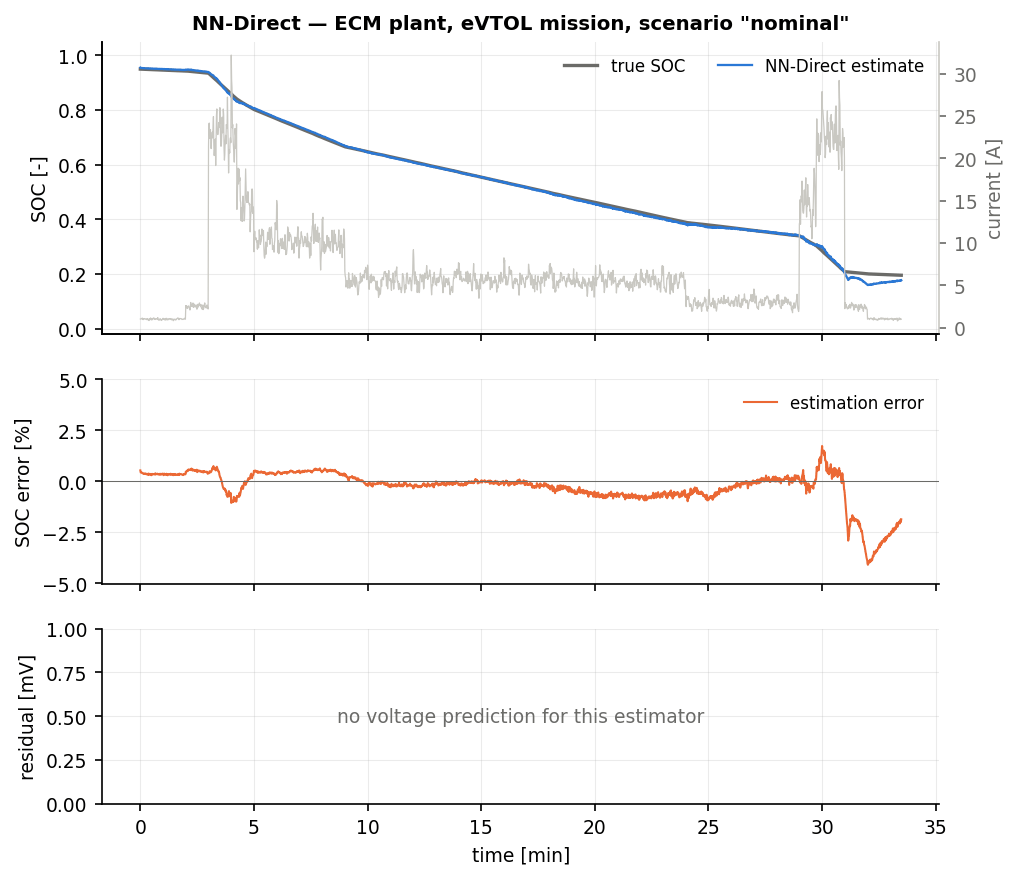
\includegraphics[width=\textwidth]{figures/cell_NNDirect_nominal.png}
\caption{NN-Direct on the nominal eVTOL mission: true and estimated SOC (top), estimation error
(middle; no $\pm2\sigma$ band is available because the method has no covariance), voltage residual
(bottom; empty --- the method makes no voltage prediction).}
\end{figure}
\begin{figure}[H]\centering
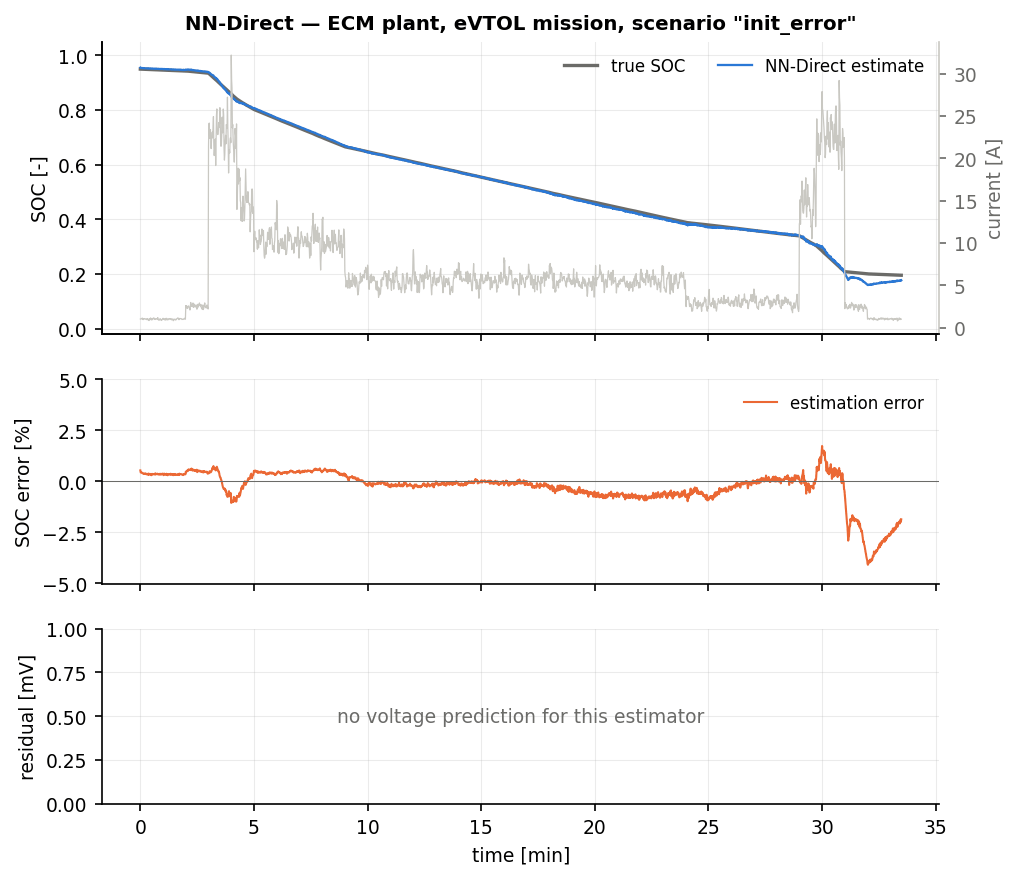
\includegraphics[width=\textwidth]{figures/cell_NNDirect_init_error.png}
\caption{NN-Direct with a \SI{35}{\percent} initial SOC error.  The trace is identical to the
nominal one: the regressor never reads the initial-SOC hypothesis, so the scenario is vacuous for
it.}
\end{figure}

All numbers below are three-seed means in per cent SOC, taken from
Table~\ref{tab:cell_NNDirect}; ``EKF ref.'' is the steady-state error of the plain EKF on the
identical data.

On the nominal eVTOL mission NN-Direct reaches $\mathrm{rmse} = \SI{0.87}{\percent}$ and
$\mathrm{rmse_{ss}} = \SI{1.17}{\percent}$ --- in line with the roughly \SI{1}{\percent} reported
by \citet{chemali2018dnn} on automotive cycles, and inside the \SI{2}{\percent} acceptance
threshold.  That is genuinely impressive for a $\num{321}$-parameter map that has never seen an
eVTOL mission.  The comparison is the bad news: the plain EKF of Chapter~\ref{ch:ekf} achieves
$\mathrm{rmse_{ss}} = \SI{0.05}{\percent}$ on the same data.  \textbf{The data-driven estimator is
twenty-three times less accurate than the model-based one on the scenario both were designed
for}, and it consumes \SI{12}{\kilo\byte} of RAM to do it.

The scenario sweep is more interesting than the headline number:
\begin{itemize}
  \item \texttt{init\_error} ($1.17$, $t_\text{conv} = \SI{0}{\second}$).  The numbers are
        \emph{bit-identical} to \texttt{nominal}, because the regressor never uses the estimator's
        initial-SOC hypothesis.  This looks like perfect robustness and is nothing of the sort: the
        network has simply memorised that these missions begin near $z_0 = 0.95$ and reconstructs
        the rest from $\Delta z^{\mathrm{CC}}$.  Start the same cell at $z_0 = 0.6$ and the feature
        $\Delta z^{\mathrm{CC}}$ is still zero at $k=0$ while the truth is not; nothing in the
        training distribution covers that case.  This is Assumption~\ref{as:nnd-cover} failing
        silently --- the most dangerous failure mode a learned component has, because the output
        stays plausible.  The same three digits reappear on \texttt{param\_mismatch} and
        \texttt{sensor\_dropout} for the same reason: those scenarios perturb the estimator's
        \emph{model}, and this estimator has none.
  \item \texttt{aged\_cell} ($1.29/1.76$, EKF ref.\ $1.52$).  The worst steady-state result of the
        sweep, and the expected one: $\Delta z^{\mathrm{CC}}$ is computed with the \emph{nameplate}
        capacity while the truth cell has lost \SI{15}{\percent}, so the feature that carries the
        integral is systematically wrong by that factor.  Aged cells were in the training set,
        which is why the error is \SI{1.8}{\percent} rather than the \SI{11}{\percent} a pure
        Coulomb count would give; the network has learned to read the remaining capacity off the
        voltage features, but only approximately.
  \item \texttt{param\_mismatch} ($0.87/1.17$ against the EKF's $1.36$) is one of only two ECM
        scenarios NN-Direct wins, and it wins by \emph{abstention}: a \SI{30}{\percent} error in
        $R_0$ is an error in a model the regressor does not have, so its output does not move at
        all.  A method with no commitments cannot be betrayed by them --- which is the same
        sentence, read the other way, as the one that explains \texttt{nominal}.
  \item \texttt{current\_bias} ($1.27$, EKF $0.61$) and \texttt{noise\_step} ($1.31$, EKF $0.12$)
        degrade mildly; \texttt{cold} ($0.69$) and \texttt{hot} ($0.30$) are the \emph{best} results
        of the sweep, because both ambient temperatures were explicitly in the training set and the
        temperature feature is used well.  Interpolation inside the training support works; that is
        the whole message.
  \item \texttt{preisach} ($0.62/0.82$, EKF $0.20$).  Half the training cells carried the Preisach
        operator, so the extra hysteresis is inside the support and the network has averaged over
        it --- but averaging is not modelling, and the result is four times the EKF's.  Compare
        NN-EKF (Chapter~\ref{ch:nnekf}), which \emph{represents} the same effect explicitly and
        reaches $0.10$, the best figure of any estimator in this report on that scenario.
  \item \texttt{combined} ($3.25/4.09$, $t_\text{conv} = \SI{79}{\second}$) is the scenario where
        NN-Direct decisively beats the EKF ($12.44$, never converging) --- a factor of three, and
        the difference between an estimator that gets inside \SI{2}{\percent} and one that does
        not.  Again the reason is abstention: the EKF is wrecked by the compounded current-sensor
        bias and capacity loss because it \emph{trusts} its model, whereas NN-Direct falls back on
        the voltage features.  The moving-horizon estimators of
        Chapters~\ref{ch:mhe} and~\ref{ch:mherti} reach \SIrange{0.5}{0.7}{\percent} on the same
        scenario, so this is a win over the EKF, not over the field.
\end{itemize}

The extrapolation hypothesis can be checked directly.  The training missions peak at
3.5\,C ($\approx\SI{17.5}{\ampere}$); the eVTOL hover segments demand 4.5\,C
with pulses to \SI{29}{\ampere}.  The per-sample error is largest exactly during the
take-off and landing hovers ($|e|_{\max} = \SI{4.2}{\percent}$ on nominal, against a steady-state
RMS of \SI{1.2}{\percent}), and the residual is signed --- the network underestimates the ohmic
drop it has never seen and therefore overestimates the SOC.  This is textbook extrapolation of a
\texttt{tanh} ridge function, which saturates instead of continuing the linear trend of $-R_0 i$.

\paragraph{Electrochemical (SPM) plant.}
\begin{figure}[H]\centering
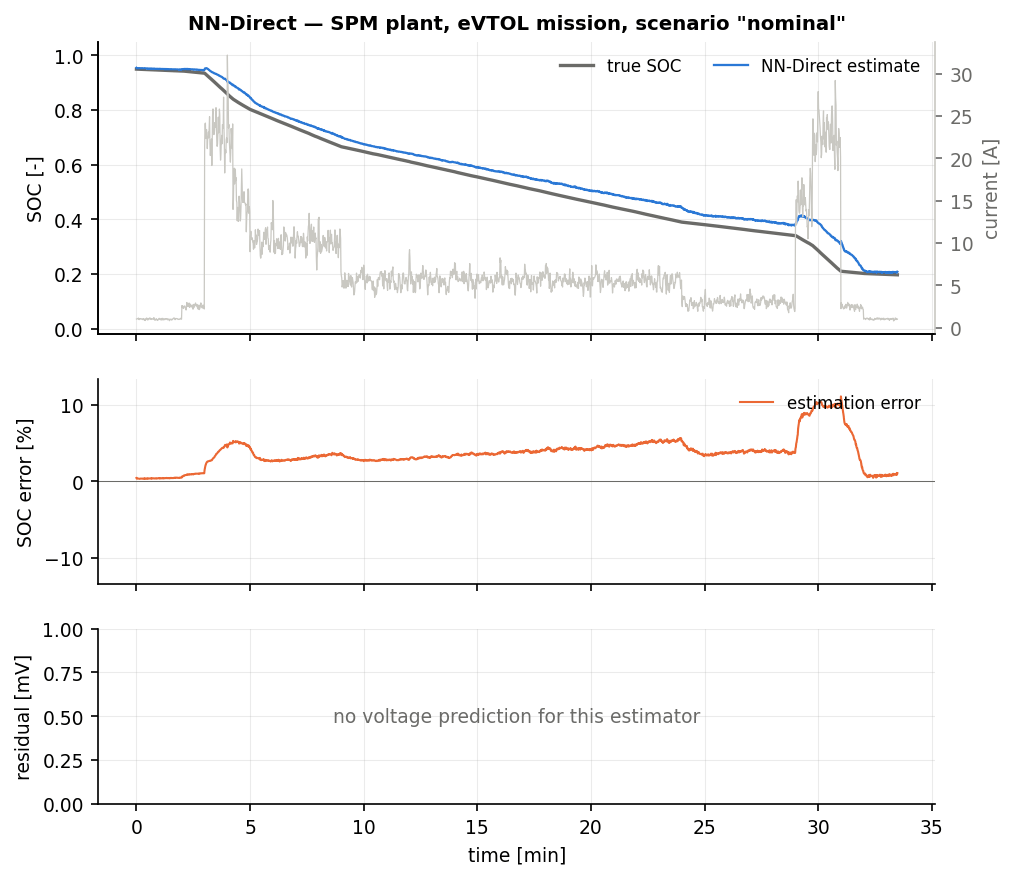
\includegraphics[width=\textwidth]{figures/cellspm_NNDirect_nominal.png}
\caption{NN-Direct on the SPM plant, nominal eVTOL mission.  The network was fitted to ECM-plant
data; the single-particle plant is a different data distribution, and the error grows by a factor
of four.}
\end{figure}
The SPM rows are the cleanest demonstration of Assumption~\ref{as:nnd-cover} in the whole report.
The truth plant is now an electrochemical single-particle model with Butler--Volmer kinetics and
slow solid diffusion ($\tau_2 = \SI{556}{\second}$), against which the estimators use a 2-RC ECM
fit that leaves a \emph{structured} \SI{4}{\milli\volt} residual.  For every model-based filter
that residual is a modelling error; for NN-Direct it is something worse --- a change of the input
distribution, because the network's voltage and moving-average features now take values it was
never trained on.  The steady-state error rises from \SI{1.17}{\percent} on the ECM plant to
\SI{5.12}{\percent} on the SPM plant, a factor of $4.4$, against the EKF's \SI{3.73}{\percent}.
Nine of the nine SPM scenarios sit between \SI{1.5}{} and \SI{5.2}{\percent}, and seven of them
report the \emph{same} $5.12$: the network's output is essentially a fixed function of the mission,
insensitive to everything the scenarios vary.  It is worth noting what plain Coulomb counting
achieves on the same plant --- \SI{0.47}{\percent}, because it never looks at the voltage at all.
The network's learned voltage corrections, trained on a different electrochemistry, are not merely
useless here; they are the thing that takes it from \SI{0.5}{} to \SI{5}{\percent}.  The two
exceptions are instructive: \texttt{cold} (\SI{1.89}{\percent} against the EKF's
\SI{7.35}{\percent}) and \texttt{current\_bias} (\SI{4.16}{} against \SI{5.69}{\percent}), where
the ECM fit is so badly wrong that having no model is again the lesser evil.

Finally, the cost: \SI{488}{\nano\second} per sample, essentially the EKF's
\SI{477}{\nano\second}, but with $30\times$ the memory and without a covariance, a voltage
prediction or a fault residual --- the \texttt{RMSE}$_v$ column of
Table~\ref{tab:cell_NNDirect} is empty for every row.  There is no operating point at which this
method is the right engineering choice for the cell-level problem \emph{as posed here}.  It becomes
attractive only where a model is genuinely unavailable --- an unknown second-life cell, a chemistry
with no published parameters --- and there its \SI{1}{\percent} accuracy with zero characterisation
effort is a real result.

\section{Summary}
NN-Direct is a faithful, deterministic, heap-free implementation of the direct-regression approach
of \citet{chemali2018dnn}, and it works: \SI{1.17}{\percent} steady-state SOC error on a mission it
has never seen, from eight measured features and $\num{321}$ weights, with no cell model at all.
It is also twenty-three times worse than an extended Kalman filter that costs the same per sample
and one thirtieth of the memory, it provides neither an uncertainty estimate nor a voltage residual,
its apparent immunity to the initial-SOC scenario is memorisation rather than robustness, and moved
to a different truth plant it degrades to \SI{5.1}{\percent} while a bare Coulomb counter on the
same data gives \SI{0.47}{\percent}.  Use it when no cell model can be obtained and the operating
envelope can be guaranteed to stay inside the training envelope; do not use it as the primary SOC
source in an airborne system, where the operating envelope is precisely what cannot be guaranteed
and where the absence of a specification to verify against is a certification obstacle rather than
an implementation detail.  Its proper role in this library is as the data-driven \emph{component}
of a hybrid --- the subject of Chapters~\ref{ch:nnekf} and~\ref{ch:elmrlsekf}.
